\chapter{Introduction}

Our objective is to develop a computational environment for the exploration
of parametric polytopes. A computational environment is one in which
we can apply rigourous defintional constraints on symbolic constructions, and
likewise manipulate them to reveal properties that may be of interest.
A parametric polytope is the union of two concepts. The first is the idea
of parameters, which are our unknown constraints in a system. The second
is a polytope, which is a some what geometric construction. We will
build an intuition of a polytope in this section, and formally define it
in the next chapter. Parameters will be applied in the computation realm
and are expanded in Section 3.


\section{A Geometric Intuition of a Polytope}

A polytope is a geometrically realizable graph composed
of linearly connected vertices\cite{Coxeter}.
A ``graph" is meant in the combinatorial sense of a structure composed of
vertices and edges that show connectivity. Thus a geometric realization
of a graph with linearly connected vertices is highly analagous to how we would traditionally
draw a graph. Figure \ref{fig:graph} shows a graph in with vertices labeled
with numbers and edges between them.

\begin{figure}[h!]
  \centering
    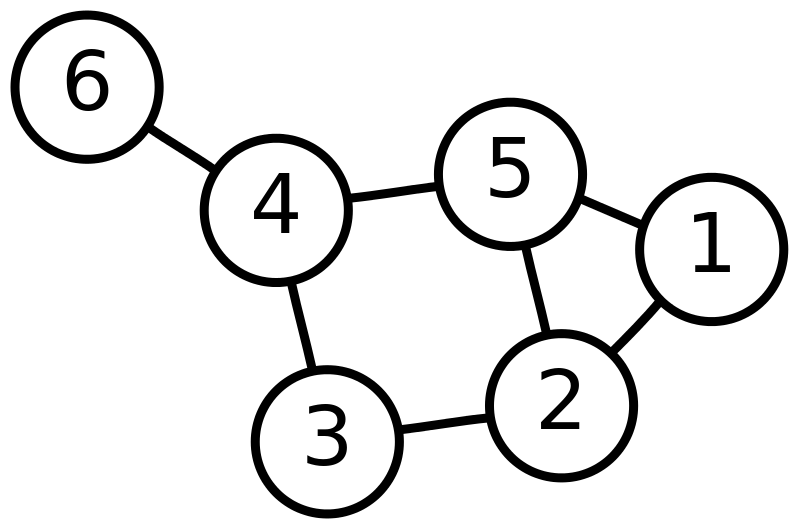
\includegraphics[width=0.5\textwidth]{img/6graph.png}
  \caption{An example of a graph.}
  \label{fig:graph}
\end{figure}

The informal term ``flat" implies the path between two vertices
on our polytope are connected by line segments. Thus for something to be
considered geometrically realizable, we must be able to assign tuple values
to the vertices. An N-polytope then exists in the corresponding euclidean
space dimension. For our purposes we will primarily use the real numbers,
$\mathbb{R}^N$, for an N-polytope.

Figure \ref{fig:polygons}
shows a two dimensional polytope, more commonly
known as a polygon. The polgons we will primarily consider are 1-cycle
graphs. 1-cycle implies that given any point there exist one path that exits
then returns to the starting point.
In three dimensions, polytopes are commonly known as a polyhedra.
Figure \ref{fig:polyhedra} shows a polyhedral representation of a dolphin.
Using this picture as reference, we see that given a vertex on a polyhedra
there may be
multiple cycles, or paths that exit then return to the vertex.
Thus many assumptions about the properties of polytopes are contigent upon
their dimensionality.
Polytopes may have properties of convexity,
connectedness,
and closure associated with them. In order to study these properties
we will illucidate a combinatoric and geometric representation
in the coming sections. More importantly we will do so rigourously!
These representations are somewhat distinct and we will see the
implications as we later develop a computational type framework.

\begin{figure}[h!]
  \centering
    
\includegraphics[width=0.75\textwidth]{img/assorted_polygons.png}
  \caption{Polygons, or two dimensional polytopes}
  \label{fig:polygons}
\end{figure}

\begin{figure}[h!]
  \centering
    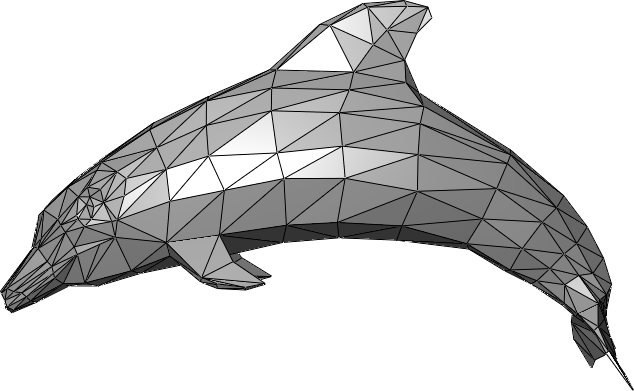
\includegraphics[width=0.75\textwidth]{img/Dolphin_triangle_mesh.png}
  \caption{A polyhedral representation of a dolphin, or a three dimensional polytope}
  \label{fig:polyhedra}
\end{figure}

\section{Flexibility of Polyhedra}

Our initial problem comes via the flexibility of polyhedra. In order to
understand flexibility of polyhedra it may be easier first to introduce the
concept of rigidity. In this case we will be concerned with 3-dimensional
polytopes, polyhedra, and observing the shape of the faces. If we give each
edge (connection between vertices) a fixed length and the freedom to pivot
around the vertex, a rigid polyhedra will not be able to deform. Cauchy's
Ridgidity theorem proves this for any convex polyhedra\cite{Gluck_1975}.
If we allow the same degrees of freedom on the edges and the shape of the
faces does not change it is called \emph{flexible}\cite{Connelly_1977}.

In 2015 Maria Hempel presented an analysis of this problem using a representation
of a polyhedra with edges and faces specified via angles and lengths
\cite{Hempel_2015}.
Such representations may be useful in a variety of dicisplines, but our
focus will be strictly structural and for enhancing the foundations for
discovering flexible polyhedra.
We will expand on the significance of this representation in later sections.

